% demo.tex
%
% Enjoy, evolve, and share!
%
% Compile it as follows:
%	xelatex demo.tex
%   bibtex demo.aux
%   bibtex lop.aux (run this, only if you pass option 'lop' below)
%   xelatex demo.tex && xelatex demo.tex
%
% Alternatively, compile it using `make -i' (see the provided Makefile).
%
% Check file `diphdthesis.cls' for other configuration options.
%
\documentclass[inscr,ack,preface]{diphdthesis}

%\usepackage{graphicx}

%%%%%%%%%%%%%%%%%%%%%%%%%%%%%%%%%%%%%%%%%%%%%%%%%%%%%%%%%%%%%%%%%%%%%%%%%%%%%%%
%%%%%%%%%%%%%%%%%%%% User-specific package inclusions %%%%%%%%%%%%%%%%%%%%%%%%%
%%%%%%%%%%%%%%%%%%%%%%%%%%%%%%%%%%%%%%%%%%%%%%%%%%%%%%%%%%%%%%%%%%%%%%%%%%%%%%%
\usepackage{booktabs}
\usepackage{hyperref}
\hypersetup{
    unicode=true,                     % non-Latin characters in bookmarks
    pdffitwindow=true,                % page fit to window when opened
    pdfnewwindow=true,                % links in new window
    pdfkeywords={},                   % list of keywords
    colorlinks=true,                  % false: boxed links; true: colored links
    linkcolor=black,                  % color of internal links
    citecolor=black,                  % color of links to bibliography
    filecolor=black,                  % color of file links
    urlcolor=black,                   % color of external links
    pdftitle={},                      % title
    pdfauthor={},                     % author
    pdfsubject={}                     % subject of the document
}
%%%%%%%%%%%%%%%%%%%%%%%%%%%%%%%%%%%%%%%%%%%%%%%%%%%%%%%%%%%%%%%%%%%%%%%%%%%%%%%
%%%%%%%%%%%%%%%%%%%% User-specific package inclusions %%%%%%%%%%%%%%%%%%%%%%%%%
%%%%%%%%%%%%%%%%%%%%%%%%%%%%%%%%%%%%%%%%%%%%%%%%%%%%%%%%%%%%%%%%%%%%%%%%%%%%%%%


%%%%%%%%%%%%%%%%%%%%%%%%%%%%%%%%%%%%%%%%%%%%%%%%%%%%%%%%%%%%%%%%%%%%%%%%%%%%%%%
%%%%%%%%%%%%%%%%%%%%%% User-specific configuration %%%%%%%%%%%%%%%%%%%%%%%%%%%%
%%%%%%%%%%%%%%%%%%%%%%%%%%%%%%%%%%%%%%%%%%%%%%%%%%%%%%%%%%%%%%%%%%%%%%%%%%%%%%%
%%%%%%%%%%%%%%%%%%%%%%%%%%%%%%%%%%%%%%%%%%%%%%%%%%%%%%%%%%%%%%%%%%%%%%%%%%%%%%%
%%%%%%%%%%%%%%%%%%%%%% User-specific configuration %%%%%%%%%%%%%%%%%%%%%%%%%%%%
%%%%%%%%%%%%%%%%%%%%%%%%%%%%%%%%%%%%%%%%%%%%%%%%%%%%%%%%%%%%%%%%%%%%%%%%%%%%%%%


%%%%%%%%%%%%%%%%%%%%%%%%%%%%%%%%%%%%%%%%%%%%%%%%%%%%%%%%%%%%%%%%%%%%%%%%%%%%%%%
%%%%%%%%%%%%%%%%%%%%%%%%%%% Required Metadata %%%%%%%%%%%%%%%%%%%%%%%%%%%%%%%%%
%%%%%%%%%%%%%%%%%%%%%%%%%%%%%%%%%%%%%%%%%%%%%%%%%%%%%%%%%%%%%%%%%%%%%%%%%%%%%%%
%
% First name, last name
%
\authorFirstGr{Ευαγγελία}
\authorFirstAbrGr{Ε.} % abbreviation of first name
\authorMiddleGr{Γ.}   % abbreviation of father's first name
\authorLastGr{Στειροπούλου}
\authorFirstEn{Evangelia}
\authorFirstAbrEn{E.}
\authorMiddleEn{G.}
\authorLastEn{Steiropoulou}

%
% The title of the thesis
%
\titleGr{Υλοποίηση Κβαντικού Μετασχηματισμού Fourier μέσω μεταβαλλόμενων κβαντικών κυκλωμάτων}
\titleEn{Implementing Quantum Fourier Transform via variational quantum circuits}

%
% Month followed by Year
%
\dateGr{ΙΟΥΛΙΟΣ 2023}
\dateEn{JULY 2023}


%
% Advisor info
%

\advisorGr{Δημήτριος Συβρίδης}
\advisorRankGr{Καθηγητής}
\advisorOrgGr{Τμήμα Πληροφορικής και Τηλεπικοινωνιών}
\advisorEn{Dimitrios Syvridis}
\advisorRankEn{Professor}
\advisorOrgEn{Department of Informatics and Telecommunications}

%
% Abstract, synopsis, inscription, ack, and preface pages.
%

\abstractEn{
    Variational quantum circuits are quantum circuits which contain gates with 
     adjustable parameters. Such circuits are already physically realizable in small scale and there is a wide
    range of possible applications for these promising structures. In this thesis, we develop the idea of tuning  a variational quantum circuit
    to simulate the important for quantum computing, operation of Quantum Fourier Transform.
    I use algebraic arguments, so called an ansatz, for reducing the depth of the variational quantum circuit 
    and I use different classical algorithms to optimize the parameters. The results of this thesis concerning 3-qubit circuits can be possibly extended to 
    a higher number of qubits.
}
\abstractGr{
    Τα μεταβαλλόμενα κβαντικά κυκλώματα είναι κυκλώματα που περιέχουν κβαντικές πύλες, με 
    παραμέτρους που μεταβάλλονται κατά τη διάρκεια της εκτέλεσης. Τα συγκεκριμένα κυκλώματα 
    είναι ήδη φυσικά εφαρμόσιμα σε μικρή κλίμακα και υπάρχει μια ευρεία γκάμα δυνατών εφαρμογών 
    για αυτά. Σε αυτήν την εργασία, αναπτύσσουμε την ιδέα της 
    υλοποίησης ενός μεταβαλλόμενου κβαντικού κυκλώματος για να προσομοιώσουμε 
    μια σημαντική για τον κβαντικό υπολογισμό 
    λειτουργία, τον Κβαντικό Μετασχηματισμό Fourier (Quantum Fourier Transform). Χρησιμοποιούμε 
    αλγεβρικά δεδομένα, έναν επονομαζόμενο ανσάτζ (ansatz) για να μειώσουμε το βάθος του 
    ποιοτικού κβαντικού κυκλώματος και χρησιμοποιούμε διάφορους κλασικούς αλγορίθμους για να 
    βελτιστοποιήσουμε τις παραμέτρους.
    Τα αποτελέσματα αυτής της εργασίας σχετικά με τα κυκλώματα τριών qubit μπορούν να επεκταθούν πιθανώς σε περισσότερα qubits.     
}
\acksEn{
}
\prefaceEn{}

\inscriptionEn{\emph{To my dear person.}}

%
% Subject area and keywords
%
\subjectAreaGr{Θεματική Περιοχή}
\subjectAreaEn{Subject Area}
\keywordsGr{Λέξη κλειδί1, λέξη κλειδί2, λέξη κλειδί3}
\keywordsEn{Keyword1, keyword2, keyword3}

%
% Set the .bib file containing your paper publications (leave the extension out)
%
% This is optional, but it should be specified when option 'lop' is passed to
% the document class.
%
% Then, inside the document environment, you may use the command '\nocitelop' to
% site your papers, as you would traditionally do with the commands '\cite' or
% '\nocite'.
%
% The papers are printed in reverse chronological order.
%
%\lopfile{mypapers/pubs}
%%%%%%%%%%%%%%%%%%%%%%%%%%%%%%%%%%%%%%%%%%%%%%%%%%%%%%%%%%%%%%%%%%%%%%%%%%%%%%%
%%%%%%%%%%%%%%%%%%%%%%%%%%% Required Metadata %%%%%%%%%%%%%%%%%%%%%%%%%%%%%%%%%
%%%%%%%%%%%%%%%%%%%%%%%%%%%%%%%%%%%%%%%%%%%%%%%%%%%%%%%%%%%%%%%%%%%%%%%%%%%%%%%

\usepackage{amsmath}
\usepackage{pdfpages}

\begin{document}

\frontmatter

% site my papers
%\nocitelop{}

\mainmatter

% add main chapters (should be given in capital letters)
\chapter{INTRODUCTION}

In the era where quantum technologies become a reality, it is useful to seek into the 
new opportunities offered to a computer scientist. While the well-known quantum algorithms
offering exponential advantage over classical ones are out of the scope of realization because of
the requiring  quantum resources, a new sort of algorithms  has emerged
which is suitable for the current experimental status and which is still promising for exhibiting a quantum advantage.
These algorithms,  the so called variational quantum algortihms (VQAs) are hybrid requiring low-depth variational  quantum circuits (VQCs) but also a classical optimization loop. VQAs are addressing different problems, using different ansatzs, but their underlined structure
is the same, resembling the one of a classical neural network where the weights/parameters are trained via a gradient descent method. 

In this work, inspired from the work ''Quantum Assisted Quantum Compiling'' we aim to train of a VQC to simulate approximately 
the effect of a circuit implementing Quantum Fourier Transform (QFT). We first build an ansatz in order to avoid to work with VQC of random structure and to  reduce the depth. Then we show that with this ansatz a relatively low-depth circuit is able to approximate the QFT on three qubits. This result if it is extensible to a higher number of qubits can be of importance, since QFT is the basic block for Shor's quantum algorithm which threatens security of RSA cryptographic scheme.
We also study another important aspect for this method and of VQA algorithms in general, that is the appropriate choice
of the classical optimization algorithm. We see that for the case under study a gradient descent method performs better
than a stochastic one.
 
 In what follows, we first provide the basic elements of a quantum circuit. Then we give some information on
the operation of a QFT and provide the initial circuit represation of it for $3$ qubits. In chapter an overview about
VQCs and VQAs is provided, while finally in chapters we present our results.

\chapter{THE BASIC ELEMENTS OF QUANTUM CIRCUITS}

Quantum circuits are a fundamental concept in quantum computation, similar to classical circuits. They consist of a sequence of quantum gates, measurements, qubit initializations, and other actions that enable quantum computation. \cite{niel}. It's important to note that quantum circuits differ from classical circuits as they operate on qubits, which can exist in superpositions of states. This allows for the exploration of multiple possibilities simultaneously, which is a key advantage of quantum computation. 

\section{Qubit}

The first thing we need to define, is the basic quantum computational unit, the qubit that is the the short for quantum bit. 
 While classical bits can only have two possible states (0 or 1), qubits can exist in a superposition of both states simultaneously. This means that a qubit can be in a linear combination of the 0 and 1 states. A qubit is a two-level quantum system, with the two basis qubit states usually represented as $\vert0\rangle$ and $\vert1\rangle$. A qubit can be in state $\vert0\rangle$, $\vert1\rangle$, or in a superposition of both states. The superposition property allows a quantum computer to be in multiple states at once, which leads to the exponential growth of possible states as the number of qubits increases.\cite{qubit}
 
 Qubit states can also be represented as vectors
 \begin{center}
 \Large
 $\vert0\rangle = 
    \begin{bmatrix}
    1 \\
    0 \\
    \end{bmatrix}$
\end{center}
\normalsize
and \\
\begin{center}
\Large
$\vert1\rangle = 
\begin{bmatrix}
0 \\
1 \\
\end{bmatrix}$
\end{center}
\normalsize
To understand the concept of a qubit, it's helpful to think about examples from the physical world. A simple analogy, is polarized light. Polarized light can be thought of as a qubit because it can be measured in two ways: vertically polarized or horizontally polarized. However, a single measurement can only give one of these two answers. In contrast, a qubit can be asked many different questions, but each question can only have one of two possible answers\cite{polarized}.

In practice, qubits are realized using various physical systems, such as the spin of an electron or the polarization of a photon. The spin of an electron is a common example of a qubit. The two levels of the electron's spin can be taken as spin up and spin down, which correspond to the 0 and 1 states of a qubit \cite{electron}. Similarly, the polarization of a single photon can be used to represent the 0 and 1 states of a qubit.

It's important to note that qubits are not limited to two-level systems. Qudits and qutrits are terms used to describe quantum systems with more than two levels. A qudit is a unit of quantum information that can be realized in suitable d-level quantum systems, where d is an integer \cite{qudit}.

The behavior of qubits is governed by the principles of quantum mechanics, such as superposition and entanglement. Superposition allows qubits to exist in multiple states simultaneously, while entanglement enables the correlation of qubits even when they are physically separated. These properties are fundamental to quantum computing and enable the potential for exponential speedup in certain computational tasks compared to classical computers.

We can use the Bloch sphere to represent the state of a single qubit. Any
state in a quantum computation can be represented as a vector that begins at
the origin and terminates on the surface of the unit Bloch sphere. By applying
unitary operators to the state vectors, we can move the state around the sphere.
We take as convention that the poles of the sphere are $\vert0\rangle$ on the top and $\vert1\rangle$ on the bottom. \cite{hidary}
We can also represent superposition states such as 
\Large $\frac{\lvert 0 \rangle + \lvert 1 \rangle}{\sqrt{2}}$ 
\normalsize as we see at the X axis.
\begin{figure}[ht]
    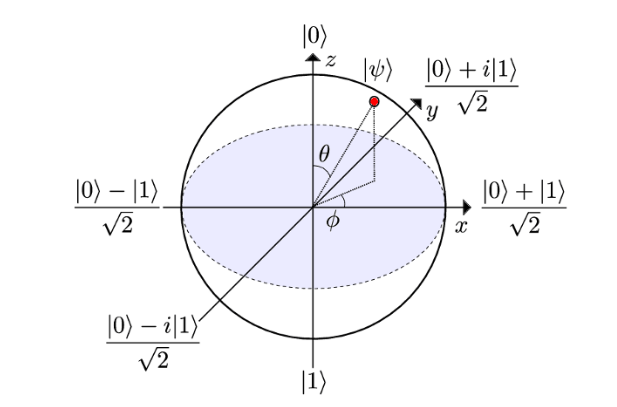
\includegraphics[width=0.9\textwidth]{bloch.png}
    \caption{The Bloch Sphere}
    \label{fig:enter-label}
\end{figure}

\cite{kockum2014quantum}


\section{Quantum Gates}

The building blocks of quantum circuits, are the quantum gates. They are operations performed on qubits, such as rotations, flips, and entanglements. Quantum gates can manipulate the quantum state of the qubits, enabling various computations and transformations. Quantum logic gates can be derived from classical logic gates, but the Hilbert-space structure of qubits allows for many quantum gates that are not induced by classical gates.

Quantum gates are described as unitary operators, represented by unitary matrices relative to some basis. The action of a quantum gate on a qubit can be represented by a matrix multiplication of the gate's unitary matrix with the qubit's state vector. Hermitian gates, such as the Pauli gates, Hadamard gate, CNOT gate, SWAP gate, and Toffoli gate, are examples of gates that are both Hermitian and unitary.

The representation of Pauli gates as matrices is the following.\cite{nielgates}
\begin{itemize}
    \item Pauli-X gate (NOT gate):
    \begin{center}
    \Large
        $X = \sigma_x = \sigma_1 = 
        \begin{bmatrix}
            0 & 1 \\
            1 & 0 \\
        \end{bmatrix}$
    \end{center}
    \normalsize
    \item Pauli-Y gate:
    \begin{center}
    \Large
        $Y = \sigma_y = \sigma_2 = 
        \begin{bmatrix}
            0 & -i \\
            i & 0 \\
        \end{bmatrix}$
    \end{center}
    \normalsize
    \item Pauli-Z gate:
    \begin{center}
    \Large
        $Z = \sigma_z = \sigma_3 = 
        \begin{bmatrix}
            1 & 0 \\
            0 & -1 \\
        \end{bmatrix}$
    \end{center}
    \normalsize
    \item Pauli-I gate (identity gate):
    \begin{center}
    \Large
        $I =  \sigma_4 = 
        \begin{bmatrix}
            1 & 0 \\
            0 & 1 \\
        \end{bmatrix}$
    \end{center}
    \item Hadamard gate:
    \begin{center}
    \Large
        $H = \frac{1}{\sqrt{2}}\begin{bmatrix}
            1 & 1 \\
            1 & -1 \\
            \end{bmatrix}$
    \end{center}
    
\end{itemize}
We will be mentioning these gates a lot as we move on in this project.
Lets study an example of the X-gate matrix applied to a qubit in state $|0\rangle$:
\Large
\begin{center}
$X|0\rangle = \begin{bmatrix}
0 & 1 \\
1 & 0 \\
\end{bmatrix}
\begin{bmatrix}
1 \\
0 \\
\end{bmatrix} = 
\begin{bmatrix}
0 \\
1 \\
\end{bmatrix} = |1\rangle$

\end{center}
\normalsize

Unlike classical logic gates, quantum gates are reversible. This means that the input state can be recovered from the output state by applying the same gate in reverse. Reversibility is a fundamental property of quantum gates and is a consequence of the unitary nature of quantum operations. Reversibility allows for the efficient simulation of classical computation using quantum circuits.

To prove it, we will apply the X-gate on the previous result, and we will notice that the initial input is the new result.

\Large
\begin{center}
$X|1\rangle = \begin{bmatrix}
0 & 1 \\
1 & 0 \\
\end{bmatrix}
\begin{bmatrix}
0 \\
1 \\
\end{bmatrix} = 
\begin{bmatrix}
1 \\
0 \\
\end{bmatrix} = |0\rangle$

\end{center}
\normalsize

\subsection{Single Qubit Gates}

In the field of quantum computing, single qubit gates and 2-qubit gates play a crucial role in manipulating and transforming the quantum states of qubits. These gates are used to perform operations on individual qubits and multiple qubits, respectively.

Starting with single qubit gates, they act on individual qubits and can be used to change their state or perform specific operations. Some commonly used single qubit gates, are the ones we mentioned before, the Pauli-X gate (bit-flip), Pauli-Y gate (bit and phase flip), Pauli-Z gate (phase flip), Hadamard gate (superposition), and the identity gate. Each of these gates is represented by a unitary matrix and operates on the state vector of a single qubit. We showed their application above. Single qubit gates can be physically realized using techniques such as laser pulses or microwave pulses to manipulate the state of individual qubits\cite{microwave}.

\subsection{2-Qubit Gates}
Moving on to 2-qubit gates, they act on two qubits simultaneously and allow for interactions between them. The controlled-NOT (CNOT) gate is a commonly used 2-qubit gate. It performs a controlled operation where the second qubit (target qubit) is flipped if and only if the first qubit (control qubit) is in the state $|1\rangle$.
    \begin{center}
    \Large
    $CNOT = 
        \begin{bmatrix}
            1 & 0 & 0 & 0 \\
            0 & 1 & 0 & 0 \\
            0 & 0 & 0 & 1 \\
            0 & 0 & 1 & 0 \\
        \end{bmatrix}$
    \end{center}
\normalsize

\begin{center}
\Large
$CNOT(|0\rangle\otimes|0\rangle) &=\begin{bmatrix} 1 & 0 & 0 & 0 \\ 0 & 1 & 0 & 0 \\ 0 & 0 & 0 & 1 \\ 0 & 0 & 1 & 0 \end{bmatrix} \begin{bmatrix} 1 \\ 0 \\ 0 \\ 0 \end{bmatrix}
&= \begin{bmatrix} 1 \\ 0 \\ 0 \\ 0 \end{bmatrix} = |00\rangle$
\end{center}
\normalsize
Lets apply the CNOT gate on \Large $|10\rangle$: \\
\begin{center}
\Large
$CNOT(|1\rangle\otimes|0\rangle)) = \begin{bmatrix}
1 & 0 & 0 & 0 \\
0 & 1 & 0 & 0 \\
0 & 0 & 0 & 1 \\
0 & 0 & 1 & 0 \\
\end{bmatrix}
\begin{bmatrix}
0 \\
0 \\
1 \\
0 \\
\end{bmatrix}
= \begin{bmatrix}
0 \\
0 \\
0 \\
1 \\
\end{bmatrix}
= |11\rangle$
\end{center}
\normalsize
As we can see, now that the control qubit is $|1\rangle$ the target qubit becomes from $|0\rangle$, $|1\rangle$.
\\
Another example of a 2-qubit gate is the Toffoli gate, which is a reversible gate that performs a NOT operation on the target qubit if both control qubits are in the state $|1\rangle$. Similar to single qubit gates, 2-qubit gates can be physically implemented using techniques such as entanglement and controlled interactions between qubits.
\begin{itemize}
\item Toffoli gate:
    \begin{center}
    \Large
    \begin{bmatrix}
        1 & 0 & 0 & 0 & 0 & 0 & 0 & 0 \\
        0 & 1 & 0 & 0 & 0 & 0 & 0 & 0 \\
        0 & 0 & 1 & 0 & 0 & 0 & 0 & 0 \\
        0 & 0 & 0 & 1 & 0 & 0 & 0 & 0 \\
        0 & 0 & 0 & 0 & 1 & 0 & 0 & 0 \\
        0 & 0 & 0 & 0 & 0 & 1 & 0 & 0 \\
        0 & 0 & 0 & 0 & 0 & 0 & 0 & 1 \\
        0 & 0 & 0 & 0 & 0 & 0 & 1 & 0 \\
    \end{bmatrix}
    \normalsize
    \end{center}
    \item Fredkin gate(controlled-swap):
    \begin{center}
    \Large
    \begin{bmatrix}
        1 & 0 & 0 & 0 & 0 & 0 & 0 & 0 \\
        0 & 1 & 0 & 0 & 0 & 0 & 0 & 0 \\
        0 & 0 & 1 & 0 & 0 & 0 & 0 & 0 \\
        0 & 0 & 0 & 1 & 0 & 0 & 0 & 0 \\
        0 & 0 & 0 & 0 & 1 & 0 & 0 & 0 \\
        0 & 0 & 0 & 0 & 0 & 0 & 1 & 0 \\
        0 & 0 & 0 & 0 & 0 & 1 & 0 & 0 \\
        0 & 0 & 0 & 0 & 0 & 0 & 0 & 1 \\
    \end{bmatrix}
\normalsize
\end{center}
\end{itemize}

In the context of quantum computing, gates can be combined in series or in parallel to create more complex operations and circuits. Series combinations of gates involve applying one gate after another, while parallel combinations involve applying gates simultaneously to different qubits. The order of gates in a circuit diagram is reversed when multiplying them together mathematically.

To sum it up, single qubit gates and 2 qubit gates are fundamental components in quantum computing. They are used to manipulate and transform the quantum states of qubits, enabling the implementation of various quantum algorithms and protocols. Single qubit gates act on individual qubits, while 2 qubit gates allow for interactions between pairs of qubits. These gates can be combined to create more complex operations and circuits, as we will see later. 

\subsection{Variational Gates}



\section{Measurements}

Measurement is another important aspect of quantum circuits. Measurements are used to extract information from qubits. They collapse the quantum state of a qubit to one of its basis states, and the measurement result is a classical value that can be used in classical computations. It's important to note that measurement in quantum mechanics is probabilistic, and the outcome of a measurement cannot be predicted with certainty.

\section{Quantum circuits}

Now using a combination of the gates mentioned before, we will create a circuit. Specifically, we will provide the a circuit, that entangles 3 qubits. As we can see, the circuit is composed of a Hadamard gate($H$), followed by two $CNOT$ gates, and lastly the measurements of the 3 qubits. \cite{ibm}
\begin{figure}[ht]
    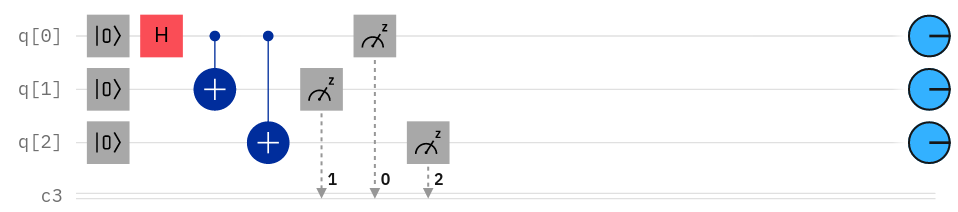
\includegraphics[width=1\textwidth]{ghz.png}
    \caption{GHZ states circuit}
    \label{fig:enter-label}
\end{figure}

GHZ states are named after Greenberger, Horne, and Zeilinger, who were the first to study them in 1989. GHZ states are also known as “Schrödinger cat states” or just “cat states.” \cite{ghz_ibm}

\chapter{QUANTUM FOURIER TRANSFORM (QFT)}

One of the most useful ways of solving a problem in mathematics or computer science is to transform it into some other problem for which a solution is known.  A great discovery of quantum computation has been that some such transformations can be computed much faster on a quantum computer than on a classical computer, a discovery which has enabled the construction of fast algorithms for quantum computers.

The Quantum Fourier Transform is a reversible transformation that operates on quantum bits (qubits) and is used to convert a quantum state from the computational basis to the Fourier basis. It is implemented using a series of unitary gates, such as the Hadamard gate and the controlled phase shift gate [1]. The QFT is particularly powerful when combined with other algorithms, as it can be used to measure the period of a function, which is essential for cracking the RSA algorithm.



\section{QFT on 3 qubits}

In terms of the circuit implementation, the QFT with 3 qubits differs from the QFT with 2 qubits in the number of gates used. The QFT with 3 qubits requires 6 gates, while the QFT with 2 qubits requires 3 gates. This means that the circuit for the QFT with 3 qubits is more complex and requires more operations compared to the circuit for the QFT with 2 qubits.

\begin{figure}[ht]
\begin{center}
    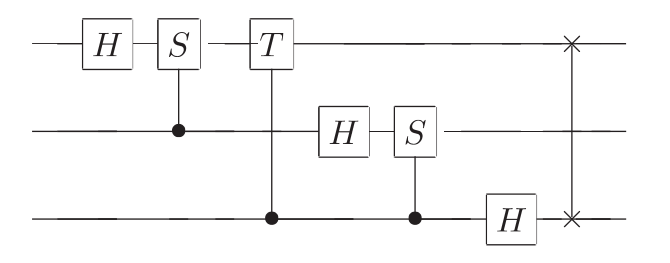
\includegraphics[width=0.75\textwidth]{qft.png}
    \caption{Quantum Fourier Transform Circuit} 
    \label{fig:enter-label}
    \end{center}
\end{figure}
\\Recall that $S$ and $T$ are the phase and π/8 gates, and $H$ is the Hadamard gate we mentioned at the beginning.\cite{niel}

\begin{itemize}
    \item S gate(phase gate):
    \begin{center}
    \Large
        \begin{bmatrix}
            1 & 0 \\
            0 & i
        \end{bmatrix}
    \end{center}
    \normalsize
    \item T gate(π/8 gate):
    \begin{center}
    \Large
    \begin{bmatrix}
    \Large
    1 & 0 \\
    0 & e^{i\pi/4}
    \end{bmatrix}
    \end{center}
\end{itemize}
\normalsize

As a matrix the quantum Fourier transform in this instance may be written out explicitly, using the following  \Large$\omega= e^{\frac{2\pi i}{8}} = \sqrt{i}$ \normalsize \cite{niel}

\Large

\[
\frac{1}{\sqrt{8}}
\begin{bmatrix}
1 & 1 & 1 & 1 & 1 & 1 & 1 & 1 \\
1 & \omega & \omega^2 & \omega^3 & \omega^4 & \omega^5 & \omega^6 & \omega^7 \\
1 & \omega^2 & \omega^4 & \omega^6 & 1 & \omega^2 & \omega^4 & \omega^6 \\
1 & \omega^3 & \omega^6 & \omega^1 & \omega^4 & \omega^7 & \omega^2 & \omega^5 \\
1 & \omega^4 & 1 & \omega^4 & 1 & \omega^4 & 1 & \omega^4 \\
1 & \omega^5 & \omega^2 & \omega^7 & \omega^4 & \omega^1 & \omega^6 & \omega^3 \\
1 & \omega^6 & \omega^4 & \omega^2 & 1 & \omega^6 & \omega^4 & \omega^2 \\
1 & \omega^7 & \omega^6 & \omega^5 & \omega^4 & \omega^3 & \omega^2 & \omega^1 \\
\end{bmatrix}
\]
$=$\[
\frac{1}{\sqrt{8}} \begin{bmatrix}
1 & 1 & 1 & 1 & 1 & 1 & 1 & 1 \\
1 & e^{i\frac{\pi}{4}} & e^{i\frac{\pi}{2}} & e^{i\frac{3\pi}{4}} & e^{i\pi} & e^{i\frac{5\pi}{4}} & e^{i\frac{3\pi}{2}} & e^{i\frac{7\pi}{4}} \\
1 & e^{i\frac{\pi}{2}} & e^{i\pi} & e^{i\frac{3\pi}{2}} & 1 & e^{i\frac{\pi}{2}} & e^{i\pi} & e^{i\frac{3\pi}{2}} \\
1 & e^{i\frac{3\pi}{4}} & e^{i\frac{3\pi}{2}} & e^{i\frac{9\pi}{4}} & e^{i\pi} & e^{i\frac{5\pi}{4}} & e^{i\frac{7\pi}{2}} & e^{i\frac{15\pi}{4}} \\
1 & e^{i\pi} & 1 & e^{i\pi} & 1 & e^{i\pi} & 1 & e^{i\pi} \\
1 & e^{i\frac{5\pi}{4}} & e^{i\frac{\pi}{2}} & e^{i\frac{7\pi}{4}} & e^{i\pi} & e^{i\frac{\pi}{4}} & e^{i\frac{\pi}{2}} & e^{i\frac{3\pi}{4}} \\
1 & e^{i\frac{3\pi}{2}} & e^{i\pi} & e^{i\frac{7\pi}{2}} & 1 & e^{i\frac{\pi}{2}} & e^{i\pi} & e^{i\frac{3\pi}{2}} \\
1 & e^{i\frac{7\pi}{4}} & e^{i\frac{3\pi}{2}} & e^{i\frac{15\pi}{4}} & e^{i\pi} & e^{i\frac{3\pi}{4}} & e^{i\frac{7\pi}{2}} & e^{i\frac{15\pi}{4}}
\end{bmatrix}
\]
\normalsize 
\\This representation of the Quantum Fourier Tranform, is going to be very useful to us, when we get to the code implementation.

\chapter{VARIATIONAL QUANTUM CIRCUITS (VQCs) AND ALGORITHMS}

\section{Variational Quantum Circuits (VQCs)}

Variational quantum circuits, also known as "parametrized quantum circuits" or "adaptable quantum circuits", are a type of quantum circuit that are used in various applications, such as supervised learning, reinforcement learning, and functional regression. They are designed to harness the potential advantages of quantum computing for solving complex problems. Variational quantum circuits involve the use of parameterized gates and measurements to encode and manipulate quantum information.

One of the main motivations behind using variational quantum circuits is to take advantage of the expressive power of quantum computing to solve problems that are difficult for classical computers. These circuits are designed to be trainable, meaning that the parameters of the gates can be adjusted to optimize the circuit's performance for a specific task. The optimization process typically involves finding the set of parameters that minimizes a cost or loss function, which is defined based on the specific problem being solved.

Variational quantum circuits can be used in different ways depending on the problem at hand. In supervised learning, for example, the circuit can be used to classify data by mapping input features to output labels. In reinforcement learning, the circuit can be used to learn policies for decision-making in partially observable environments. In functional regression, the circuit can be used to approximate the relationship between input and output variables.

One common approach in variational quantum circuits is to use a hybrid model that combines classical and quantum components. This allows for the use of classical optimization algorithms to update the parameters of the circuit based on feedback from the classical part of the model. This hybrid approach helps to mitigate the noise and errors inherent in current quantum hardware, known as NISQ (Noisy Intermediate-Scale Quantum) devices.

The encoding scheme used in variational quantum circuits depends on the specific problem and the type of circuit being used. Different types of circuits, such as Type 1, Type 2, and Type 3, have different ways of encoding the input data. For example, Type 1 circuits encode the input as complex-valued numbers, while Type 2 circuits encode the input using binary representation. The choice of encoding scheme can affect the performance and efficiency of the circuit for a given problem.

The training process of variational quantum circuits involves updating the parameters of the gates using gradient descent optimization. The gradients of the loss function with respect to the circuit parameters are calculated using the backpropagation method, similar to the calculation in classical neural networks. The gradients are then used to update the parameters in the direction that minimizes the loss function.

The performance of variational quantum circuits can be evaluated through numerical simulations and experiments on quantum hardware. Simulations can provide insights into the learning performance and efficiency of the circuits, while experiments on real quantum machines, such as IBMQ systems, can test the applicability and scalability of the circuits in real-world scenarios.

Variational quantum circuits are still an active area of research, and there are ongoing efforts to explore their capabilities and limitations. Theoretical analysis, such as error performance analysis and optimization properties, can provide insights into the representation and generalization powers of variational quantum circuits. Experimental validation on different datasets and problem domains is crucial for understanding the practical usefulness of these circuits.

In conclusion, variational quantum circuits are a promising approach for leveraging the power of quantum computing in solving complex problems. They involve the use of parameterized gates and measurements to encode and manipulate quantum information. By training the circuits using classical optimization algorithms, variational quantum circuits can potentially outperform classical methods in certain applications. However, further research and experimentation are needed to fully understand and harness the capabilities of variational quantum circuits.

\section{Variational Quantum Algorithms (VQAs)}

Variational quantum algorithms (VQAs) are a type of hybrid quantum-classical optimization algorithm that harnesses the capabilities of both classical and quantum computers to solve complex problems. VQAs have emerged as a promising approach in the Noisy Intermediate-Scale Quantum (NISQ) era, where quantum computers are characterized by noise and imperfections. These algorithms involve evaluating an objective function using a parameterized quantum circuit and updating the parameters of the circuit using classical optimization methods. VQAs have found applications in various domains, including quantum chemistry, quantum simulations, optimization problems, and quantum machine learning [1].

In VQAs, the objective function is typically encoded by a parameterized quantum circuit, which serves as an ansatz or guess for the ground state of the system. The quantum computer evaluates the objective function by measuring the expectation value of an observable, often the Hamiltonian of the system. The classical optimizer then utilizes this evaluation to update the parameters of the circuit, aiming to minimize the associated cost function. Classical optimization methods such as gradient descent can be employed to iteratively adjust the parameters and approach the optimal solution [1].

The noise and errors inherent in current quantum hardware present challenges for implementing VQAs. NISQ devices are prone to errors, and the probability of failed operations is non-negligible. Consequently, VQAs often rely on shallow circuits or circuits with a significant fraction of failed operations to ensure reliability. However, this limitation can impact the performance of VQAs and restrict their effectiveness in the presence of noise [3].

The concept of quantum advantage is relevant to VQAs. Quantum advantage refers to the ability of a quantum algorithm to solve certain problems more efficiently or faster than classical algorithms. However, the extent of quantum advantage depends on the specific problem being solved and the capabilities of the quantum hardware. For certain optimization problems, achieving quantum advantage may require circuits with a depth that scales at least logarithmically with the system size [3].

In conclusion, variational quantum algorithms are hybrid quantum-classical optimization algorithms that leverage the power of both classical and quantum computers. They involve evaluating an objective function using a parameterized quantum circuit and updating the parameters using classical optimization methods. VQAs have applications in quantum chemistry, quantum simulations, and optimization problems. However, the presence of noise and the limitations of current quantum hardware can affect their performance. The extent of quantum advantage achieved by VQAs depends on the specific problem and the capabilities of the quantum hardware [1][3].


\chapter{ QFT VIA A  VQC WITH 3 qubits}

As we mentioned before, QFT is an essential operation in quantum computing. To be realized for $n$ qubits this requires 
$\approx n^2$ gates that is an excellent record --taking into account that a general unitary operation
is described by $4^n$ real parameters. On the other hand, this includes controlled-phase gates $R_n$
each of which if to be decomposed into gates from a universal set, requires with the best known
method up today $\approx 20$ gates and an ancillary qubit. 

In the NIST era the idea of employing fault-tolerant quantum computation has been set aside
since deep-depth circuits are out of discussion. In this work we investigate the question
of realizing the QFT operation with a variational circuit of relatively low depth. Instead of
working with universal set of gates we employ Hamiltonians which can be in principle physically realizable.
 The initial procedure that we follow for a $3$-qubit is a standard one:
\begin{itemize}
	\item We build an ansantz on the structure of the circuit based on the algebraic properties of QFT.
	\item We define a cost function that measures the distance from the target operation i.e. QFT.
	\item We optimize the parameters in the circuit with a stochastic gradient descent so that the cost is minimized. 
\end{itemize}
At second stage, we minimize as possible the depth of the circuit and we update the cost function to an experimentally accessible one.
Naturally in order to arrive to useful results we try to generalize working with $4$ and $5$ qubit circuits.
  
\section{Building an Ansanz} 

In order to build an ansatz we first take the unitary matrix (in the computational basis), $\hat{U}_{QFT}$,
and we decompose it onto the $64$ generators of $SU(8)$ algebra, i.e. $\hat{g}_{ijk}=\hat{\sigma}_{i} \otimes \hat{\sigma}_{j} \otimes \hat{\sigma}_{k}$,
as 
\begin{equation}
O_{ijk}=Tr\left(\hat{U}_{QFT} \hat{g}_{ijk} \right).
\end{equation}
The $\hat{\sigma}_{i}$ with $i=1,2,3$ are the Pauli matrices for a single qubit while $\hat{\sigma}_{4}=\hat{1}$.

We find out (see mathematica file) that only $20$ generators give non-zero overlap $O_{ijk}$.

We commute these $20$ generators and we find out that these together with first, second,.. order commutations form
a closed subgroup of $32$ elements. Then we search for a minimum set of single-qubit and two-qubit operators able to generate the whole
subgroup. We identify $11$ of them ($5$ single qubit and $6$ two-qubit Hamiltonians) but possibly this result could be improved.

We build a parametrized circuit with these $N=11$ operators, e.g. $\hat{U}_{ijk}\left(\phi\right)=\left(-I \phi \hat{g}_{ijk}\right)$ and we search to optimize the $11$ angles $\vec{\phi}=\left\{\phi_1,\ldots, \phi_{11}\right\}$ so that the cost function is as low as possible:
\begin{equation}
C\left(\hat{U}_c\left(\vec{\phi}\right), \hat{U}_{QFT}\right)=1-\frac{1}{64}\left|Tr\left(\hat{U}_c\left(\vec{\phi}\right)\hat{U}_{QFT}^{\dagger} \right)\right|^2
\end{equation}
where $\hat{U}_c\left(\vec{\phi}\right)$ represents the unitary of the variational circuit.

The results of some preliminary tests:
\begin{itemize}
	\item $N=11$, minimum $C=0.6$
	\item $N=22$, minimum $C=0.038$
	\item $N=29$, minimum $C=0.00005$.
\end{itemize}
From these we conclude that for a good approximation the depth cannot be as low as desired.
On the other hand when I replace the two-qubit operations with random ones (from the set of $64$ generators) the 
results much deteriorate which exhibits the fact that the ansatz is strong. For instance I get for $N=29$, minimum $C=0.074$.

Much left to be done and to be investigated but at first look there is some promise, having double two-qubit operations
than the initial circuit but the flexibility to work with physical operations than rigid CNOT gates.
The essence of the method will be in the scaling.


\section{Gradient Descent Optimizer}

Before we move on to the code implementation, it is important to give some information about the optimization method I used for this project. 

Gradient descent is an iterative optimization algorithm used to find the local minimum of a differentiable function. It is particularly useful in machine learning for minimizing the cost or loss function [2]. The basic idea behind gradient descent is to take repeated steps in the opposite direction of the gradient (or approximate gradient) of the function at the current point, because this is the direction of steepest descent. By iteratively updating the parameters in the direction of the negative gradient, the algorithm gradually converges towards a minimum point [2].

To understand gradient descent, let's consider an analogy. Imagine a person who is stuck in the mountains and is trying to find the lowest point (i.e., the global minimum). Due to heavy fog, the person cannot see the path down the mountain. Instead, they must rely on local information to find the minimum. In this scenario, the person can use the method of gradient descent. They look at the steepness of the hill at their current position and proceed in the direction with the steepest descent (i.e., downhill). If they were trying to find the top of the mountain (i.e., the maximum), they would proceed in the direction of steepest ascent (i.e., uphill) [2].

In the context of machine learning, gradient descent is used to update the parameters of a model in order to minimize the cost or loss function. The parameters refer to the coefficients in linear regression or the weights in neural networks [9]. The goal is to find the parameter values that minimize the cost function, which represents the discrepancy between the predicted values and the actual values in the training data [8].

There are different variations of gradient descent, including batch gradient descent, mini-batch gradient descent and stochastic gradient descent, which is also tested in this project.

    Stochastic Gradient Descent: In stochastic gradient descent, the algorithm calculates the gradient of the cost function with respect to a single training example in each iteration and updates the parameters based on this gradient. This method is computationally efficient but can have high variance in the parameter updates, leading to slower convergence. However, it can escape local minima and find better solutions [9].

The choice of which variation of gradient descent to use depends on the specific problem and the available computational resources. Batch gradient descent is typically used when the dataset can fit into memory and computational efficiency is not a major concern. Stochastic gradient descent and mini-batch gradient descent are often preferred for large datasets or when computational efficiency is important [9].

In summary, gradient descent is an iterative optimization algorithm used in machine learning to minimize the cost or loss function. It updates the parameters of a model by taking steps in the opposite direction of the gradient of the cost function. Different variations of gradient descent, such as batch gradient descent, stochastic gradient descent, and mini-batch gradient descent, offer trade-offs between computational efficiency and convergence speed. The choice of which variation to use depends on the specific problem and available computational resources [2][8][9].

\chapter{RESULTS}
Multiple tests were run. Some plots with results are provided bellow.

You need to provide a circuit structure.

\section{Gradient Descent Results}

Firstly I tested the program with \textbf{18 parameters}.\\

\begin{figure}[ht]
\begin{center}
    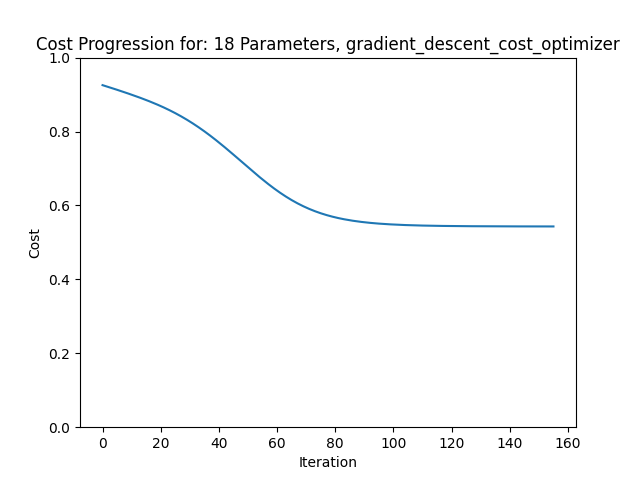
\includegraphics[width=0.9\textwidth]{plots/18.png}
    \caption{Cost progression plot, with 18 learnable parameters, using Gradient Descent optimizer} 
    \label{fig:enter-label}
    \end{center}
\end{figure}

It is obvious, that in this particular snapshot, the final cost is not the optimal result.
\\Here are the initial and the final parameters, as well as the initial and final costs. 
\\\\\textbf{X INITIAL} is:
 tensor([1.7658, 3.4312, 4.1421, 5.3068, 0.1327, 5.7904, 4.1582, 1.2668, 5.6374,
        6.0970, 2.9710, 1.6479, 0.6261, 2.5107, 3.8973, 3.1691, 0.1296, 4.8192])
\\
\textbf{initial cost}: tensor(0.9279)
\\\\\textbf{X FINAL} is:
 tensor([1.4667, 4.2022, 4.2278, 5.2510, 0.1786, 6.2554, 3.9019, 1.3128, 5.7231,
        6.0693, 3.4226, 1.6939, 0.3527, 2.5964, 4.2336, 2.5559, 0.2154, 4.8651]),

\textbf{final cost}: tensor(0.5432)

learning rate =  0.05\\ 
delta =  0.005 \\
epsilon =  1e-08 \\
threshold =  1e-05 \\
step size =  0.1 \\
\\More information about how the code is implemented, are in the appendix.

Some other implementations with 18 parameters gave similar results.
\begin{itemize}
    \item \textbf{18 parameters, b } :
    
learning rate =  0.05 \\
delta =  0.005 \\
epsilon =  1e-06 \\
threshold =  0.001 \\
step size =  0.1 \\

\textbf{X INITIAL} is:
 tensor([5.1366, 3.9022, 2.4849, 1.1003, 4.8399, 0.5321, 3.2011, 1.7677, 2.4073,
        0.9287, 4.7974, 4.5628, 4.7718, 6.1509, 5.1577, 5.5043, 0.7340, 4.3147])

\textbf{initial cost}: tensor(0.9331)

\textbf{X FINAL} is:
 tensor([5.3453, 3.5565, 2.4805, 1.2529, 4.8025, 0.6241, 3.3325, 1.7303, 2.4029,
        1.2196, 4.7847, 4.5254, 4.7614, 6.1465, 4.9526, 5.4006, 0.7295, 4.2773])

\textbf{final cost}: tensor(0.7963)

\item \textbf{18 parameters, c }:

\textbf{X INITIAL} is:
 tensor([4.5020, 3.6611, 4.0598, 2.9111, 2.0045, 5.8821, 0.1404, 0.9037, 5.4573,
        1.2292, 1.0254, 4.8697, 4.4681, 4.1592, 4.2880, 4.0359, 1.9999, 2.4546])

\textbf{initial cost}: tensor(0.9809)

\textbf{X FINAL is}:
 tensor([4.5905, 4.2028, 4.1168, 2.4467, 2.2443, 6.2634, 0.7550, 1.1436, 5.5143,
        1.0207, 1.2979, 5.1095, 5.0702, 4.2162, 4.2512, 4.1232, 2.0569, 2.6944])

\textbf{final cost}: tensor(0.5431)

\end{itemize}

After multiple executions with 18 parameters, I realized that the final cost would not get lower than 0.5. As a result, more parameters are needed to train this circuit and minimize the cost. 

Lets test the program with \textbf{20 parameters}: 

\begin{figure}[ht]
\begin{center}
    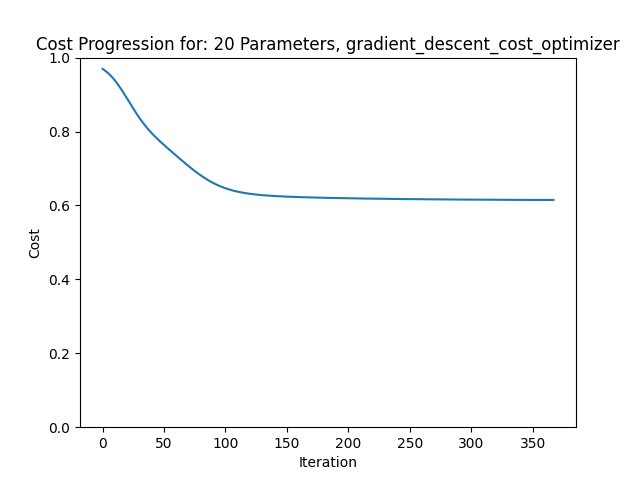
\includegraphics[width=0.9\textwidth]{20.png}
    \caption{Cost progression plot, with 20 learnable parameters, using Gradient Descent optimizer} 
    \label{fig:enter-label}
    \end{center}
\end{figure}

\textbf{X INITIAL} is: tensor([3.1948, 5.3759, 4.9216, 0.6639, 0.7274, 1.3457, 4.1867, 3.4602, 3.4542,
        3.5626, 2.9046, 5.0324, 1.6932, 1.5336, 2.8378, 5.3266, 2.7702, 1.1606,
        1.8269, 0.3608])

\textbf{initial cost}: tensor(0.9716)

\textbf{X FINAL} is: tensor([2.8576, 5.6991, 5.1387, 0.9144, 0.7338, 1.1805, 3.8612, 3.4666, 3.6713, 3.6662, 3.3033, 5.0389, 2.3572, 1.7507, 3.0914, 4.9087, 2.9874, 1.1671, 1.9527, 1.1274])

\textbf{final cost}: tensor(0.6147)


After multiple executions, I concluded that I need to increase the parameters a little more, since 20 parameters are not enough.

\begin{itemize}
    \item \textbf{22 parameters}:

\begin{figure}[ht]
\begin{center}
    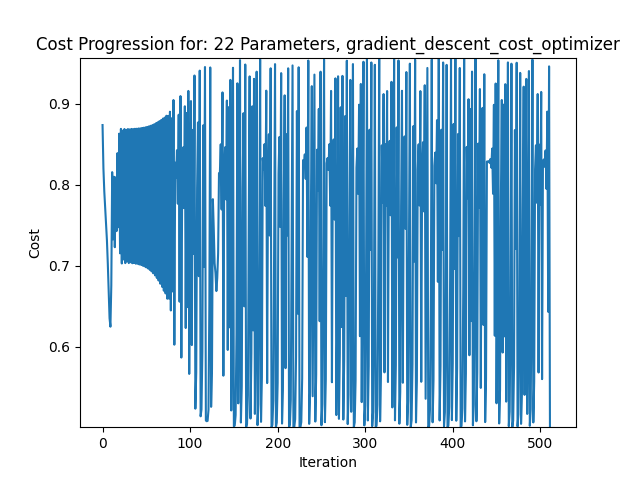
\includegraphics[width=0.9\textwidth]{plots/22.png}
    \caption{Cost progression plot, with 22 learnable parameters, using Gradient Descent optimizer} 
    \label{fig:enter-label}
    \end{center}
\end{figure}

\textbf{X INITIAL} is: tensor([4.9691, 4.7639, 2.1722, 2.4414, 4.4904, 4.0520, 3.8530, 5.6306, 1.7001,
        4.0501, 0.9469, 3.2963, 1.8443, 1.3293, 3.3896, 2.9523, 2.7749, 4.9275,
        1.4383, 4.3189, 4.7543, 2.8610])
        
\textbf{initial cost}  = tensor(0.9359)

\textbf{X FINAL} is: tensor([5.6587, 3.9270, 2.1907, 1.9635, 4.5680, 3.5704, 3.9270, 5.7082, 1.7185,
        4.7124, 0.6390, 3.3739, 2.0138, 1.3477, 3.4034, 2.5525, 2.7933, 5.0051,
        1.5708, 4.2347, 4.9088, 1.9635])

\textbf{final cost} = tensor(0.5000)

\item \textbf{26 parameters, a}:

\begin{figure}[ht]
\begin{center}
    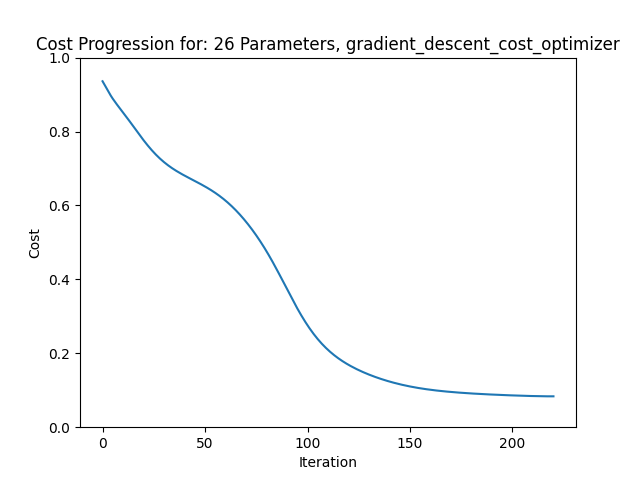
\includegraphics[width=0.9\textwidth]{26.png}
    \caption{Cost progression plot, with 26 learnable parameters, using Gradient Descent optimizer} 
    \label{fig:enter-label}
    \end{center}
\end{figure}

\textbf{X INITIAL} is:
 tensor([3.2022, 5.6416, 4.8515, 3.3115, 3.6187, 5.0852, 2.9730, 5.0537, 1.5072,
        4.7531, 0.5125, 5.5763, 5.8622, 1.1606, 0.6496, 2.2168, 3.9991, 5.3104,
        4.2755, 3.8328, 1.0954, 1.9451, 4.8207, 4.8218, 4.6000, 1.4309])

\textbf{initial cost}: tensor(0.9451)

\textbf{X FINAL} is: 
 tensor([2.3827, 5.2529, 4.6696, 3.5108, 3.6095, 5.0535, 3.9956, 5.2220, 1.1325,
        4.1914, 0.7261, 5.7447, 5.8750, 0.7859, 0.9014, 2.5525, 3.6244, 5.4788,
        3.8632, 4.2661, 0.9771, 2.2849, 5.1514, 4.4313, 4.2616, 1.4216])

\textbf{final cost} : tensor(0.0836)

learning rate =  0.05 \\
delta =  0.005 \\
epsilon =  1e-08 \\
threshold =  0.0001\\ 
step size =  0.1 \\

After testing the circuit for 18, 20 and 22 parameters, on 26 parameters the result is optimal. The cost is minimized and is equal to 0.0836.


\item \textbf{26 parameters, b}:

\begin{figure}[ht]
\begin{center}
    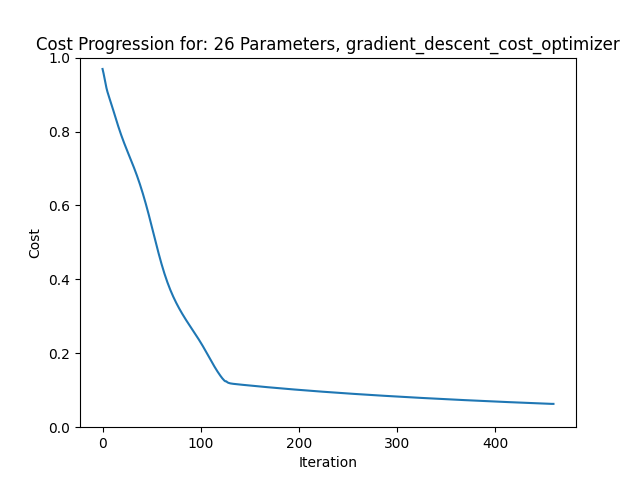
\includegraphics[width=0.9\textwidth]{26_b.png}
    \caption{Cost progression plot, with 26 learnable parameters(b), using Gradient Descent optimizer} 
    \label{fig:enter-label}
    \end{center}
\end{figure}

\textbf{X INITIAL} is:
 tensor([2.8648, 5.4188, 0.7875, 4.8503, 4.0227, 1.7765, 1.3553, 0.6937, 5.7583,
        0.8078, 4.9534, 1.9077, 6.2795, 0.9409, 3.3676, 0.6460, 3.6312, 4.4370,
        5.8479, 5.9351, 5.4692, 2.7993, 3.0437, 3.2066, 5.3126, 2.4545])
        
\textbf{initial cost}: tensor(0.9781)

\textbf{X FINAL} is:

tensor([3.3034, 5.5917, 0.8085, 4.6238, 4.3980, 1.5872, 0.9654, 0.7109, 5.4160,
        1.0719, 4.8915, 1.9250, 5.3130, 0.5986, 4.1386, 0.9808, 3.2889, 4.4543,
        5.9470, 5.9129, 5.4806, 2.7109, 3.6705, 2.8900, 5.2372, 2.8299])

\textbf{final cost}: tensor(0.0631)

learning rate =  0.05 \\
delta =  0.005 \\
epsilon =  1e-08 \\
threshold =  0.0001\\ 
step size =  0.1 \\

\item \textbf{26 parameters, c}:

\textbf{X INITIAL} is:
 tensor([6.1234, 5.7969, 2.5003, 0.5580, 5.0908, 4.7843, 2.4722, 1.7875, 5.8223,
        2.4807, 4.6223, 1.6604, 4.6718, 4.6132, 0.8379, 0.9381, 1.7933, 5.8322,
        5.2766, 4.0728, 3.6663, 1.7227, 1.2303, 3.9384, 4.3709, 4.5244])
        
\textbf{initial cost}: tensor(0.9262)

\textbf{X FINAL} is:

 tensor([5.9466, 5.8995, 2.5525, 0.6608, 4.7011, 5.4972, 2.5109, 2.6193, 5.6731,
        2.4827, 4.0413, 2.4922, 4.4677, 4.4639, 0.3543, 0.9818, 1.6441, 6.6640,
        5.4211, 4.3279, 3.1420, 1.3268, 1.5708, 3.8691, 4.0381, 4.1347])

\textbf{final cost}: tensor(0.0575)

learning rate =  0.05 \\
delta =  0.005 \\
epsilon =  1e-08 \\
threshold =  0.0001\\ 
step size =  0.1 \\

\item \textbf{28 parameters,  a}: 

\begin{figure}[h]
\begin{center}
    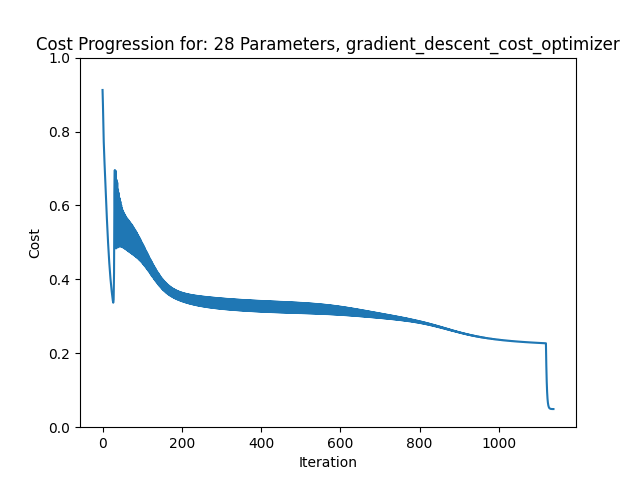
\includegraphics[width=0.9\textwidth]{28.png}
    \caption{Cost progression plot, with 28 learnable parameters, using Gradient Descent optimizer} 
    \label{fig:enter-label}
    \end{center}
\end{figure}

\textbf{X INITIAL} is:
 tensor([3.6285, 0.5717, 1.3463, 0.2393, 3.4633, 1.5723, 6.1080, 5.0117, 4.5497,
        1.1938, 5.7585, 1.8747, 2.4548, 3.4901, 4.9434, 3.3576, 0.2792, 4.1673,
        3.8621, 2.6452, 4.2201, 5.2078, 4.3327, 5.5728, 5.9729, 0.1138, 2.8426,
        4.2832])
        
\textbf{initial cost}: tensor(0.9368)

\textbf{X FINAL} is:
tensor([ 2.7217,  0.4280,  0.1943,  0.3745,  3.3493,  1.4766,  6.7955,  5.2375,
         4.6558,  0.7024,  5.9003,  2.1004,  2.4367,  3.5962,  3.9115,  3.3380,
         0.3853,  4.3931,  3.5211,  2.5860,  3.9345,  5.3438,  3.9282,  5.4054,
         5.5653, -0.0083,  3.1441,  4.0902])

\textbf{final cost}: tensor(0.0491)

learning rate =  0.05 \\
delta =  0.005 \\
epsilon =  1e-08 \\
threshold =  0.0001\\ 
step size =  0.1 \\

\item \textbf{28 parameters,  b}: 

\textbf{X INITIAL}  is:
 tensor([5.4860, 0.9125, 4.8773, 2.8955, 2.7465, 3.9753, 4.7699, 0.2627, 6.0902,
        4.7684, 5.9787, 3.1965, 1.6134, 5.1578, 5.2677, 1.9755, 1.4814, 1.6307,
        5.5425, 5.2327, 1.3015, 4.7017, 4.4076, 0.9839, 1.0343, 4.2678, 5.6086,
        0.2922])
        
\textbf{initial cost}: tensor(0.9718)

\textbf{X FINAL} is:
 tensor([5.4056, 1.1386, 5.2554, 3.3732, 3.0859, 3.8198, 5.5777, 0.0136, 5.9092,
        4.4720, 5.4650, 2.9474, 1.6145, 4.9768, 5.3171, 2.5533, 1.3004, 1.3816,
        5.6967, 5.1791, 1.6984, 4.7156, 4.8104, 0.9674, 0.6554, 4.1619, 5.3412,
        0.1582])

\textbf{final cost}: tensor(0.1112)

learning rate =  0.05 \\
delta =  0.005 \\
epsilon =  1e-08 \\
threshold =  0.0001\\ 
step size =  0.1 \\

\end{itemize}

\section{Stochastic Gradient Descent Results}

\chapter{CONCLUSIONS AND FUTURE WORK}

\section{Conclusions}


\chapter{APPENDIX}
\section{Mathematica implementation}
\section{Python implementation}

This project is implemented in python, using mostly the \textbf{PyTorch} library. 


I also implemented gradient descent, as well as stochastic gradient descent by hand, since the optimizers included in pytorch library, were not suitable for this type of model. The final circuit is a $8\times8$ matrix, that is imposible to be optimized by using simply the \textbf{torch.optim} package.\\

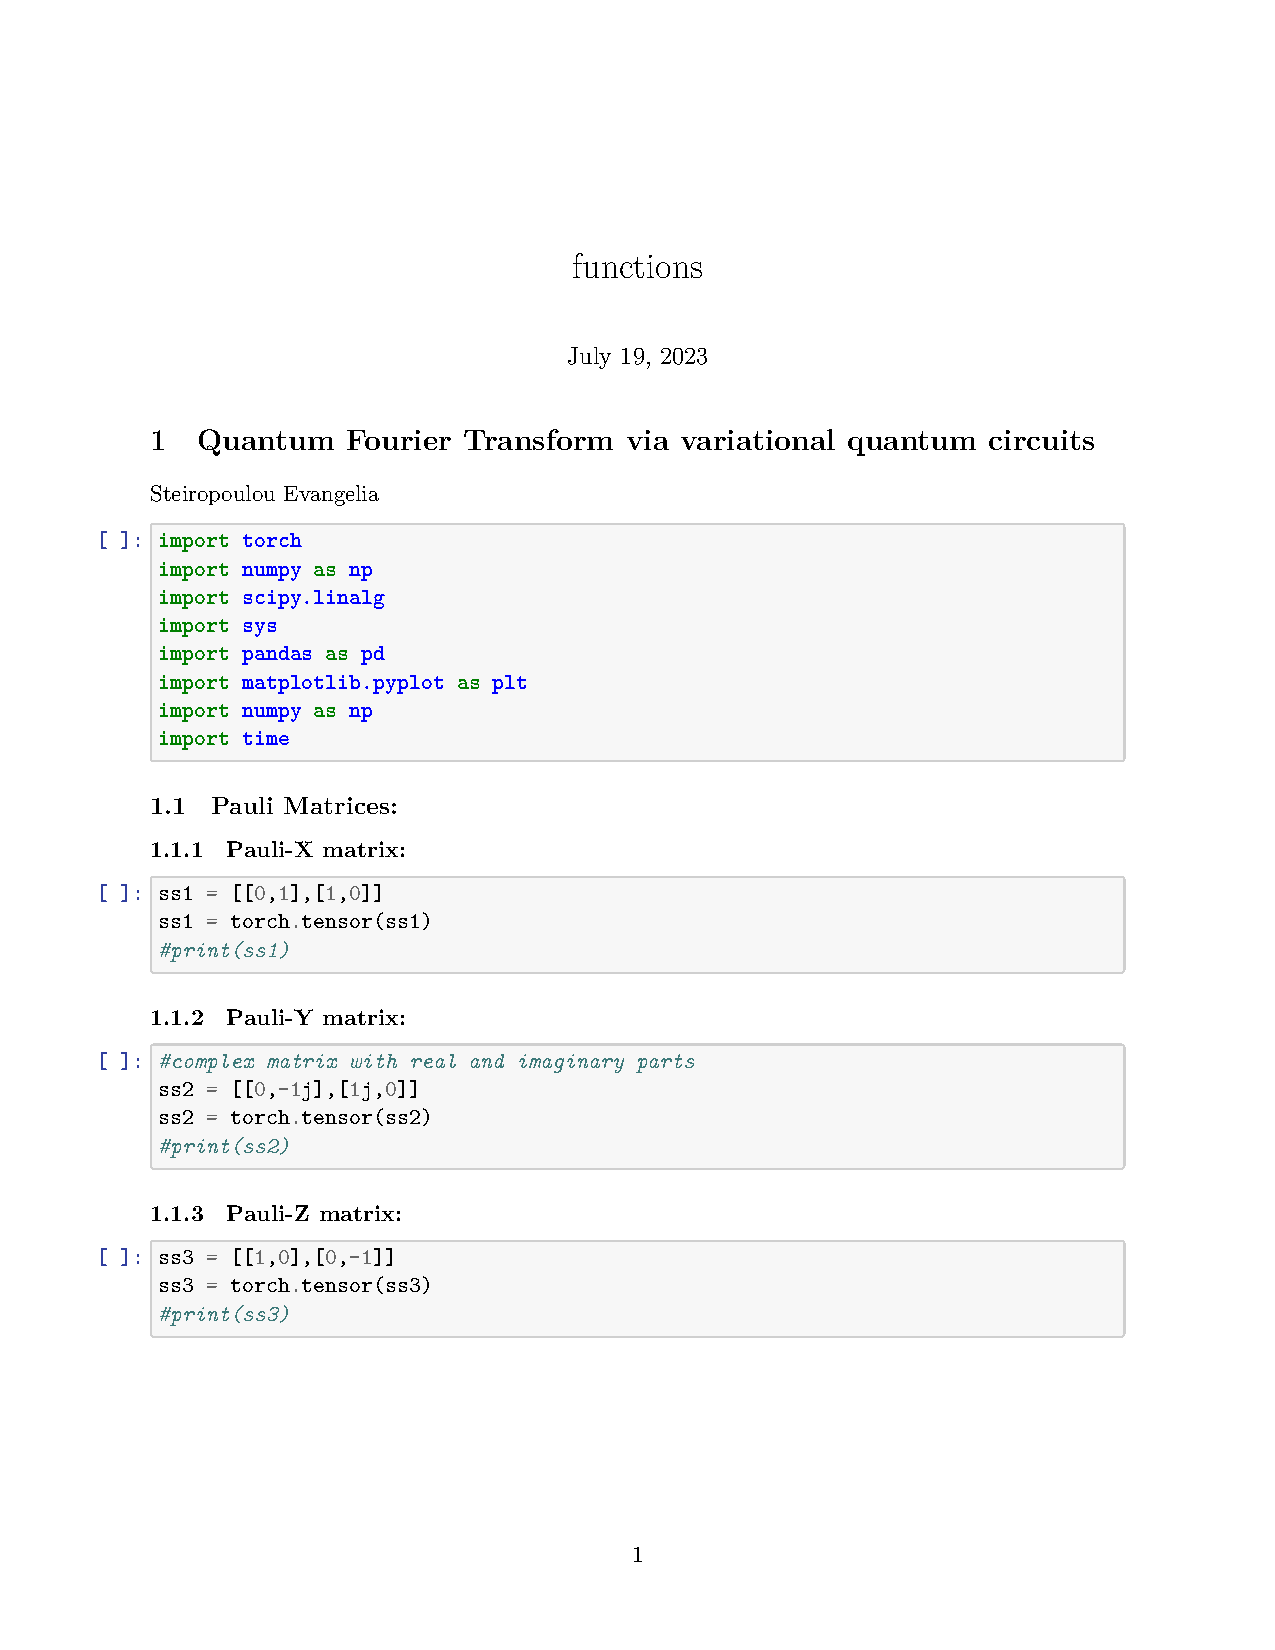
\includepdf[pages=-]{functions.pdf}

% manually include the bibliography
\bibliographystyle{plain}
\bibliography{references}

\begin{thebibliography}{99}                                                                     
\bibitem{niel}Nielsen, M. \& Chuang, I. Quantum computation and quantum information. (Cambridge university press,2010)
\bibitem{qubit}https://www.quantum-inspire.com/kbase/what-is-a-qubit/
\bibitem{polarized}https://arstechnica.com/science/2010/01/a-tale-of-two-qubits-how-quantum-computers-work/
\bibitem{nielgates}Nielsen, M. \& Chuang, I. Quantum computation and quantum information. (Cambridge university press,2010)
\bibitem{electron}https://www.techtarget.com/whatis/definition/qubit
\bibitem{qudit}Wang, Y., Hu, Z., Sanders, B. \& Kais, S. Qudits and high-dimensional quantum computing. {\em Frontiers In Physics}. \textbf{8} pp. 589504 (2020)
\bibitem{hidary}Hidary, J. \& Hidary, J. Quantum computing: an applied approach. (Springer,2019)
\bibitem{kockum2014quantum}Kockum, A. Quantum optics with artificial atoms. (Chalmers Tekniska Hogskola (Sweden),2014)
\bibitem{microwave}Gaebler, J., Tan, T., Lin, Y., Wan, Y., Bowler, R., Keith, A., Glancy, S., Coakley, K., Knill, E., Leibfried, D. \& Others High-fidelity universal gate set for be 9+ ion qubits. {\em Physical Review Letters}. \textbf{117}, 060505 (2016)
\bibitem{ghz}Mermin, N. What's wrong with these elements of reality?. {\em Physics Today}. \textbf{43}, 9-11 (1990)
\bibitem{ibm}https://quantum-computing.ibm.com/composer/files/7485fbf8fdd965ddc4a57e69ae67655d60d8b46d5e25f74650d993176f36b35c
\bibitem{ghz_ibm}https://quantum-computing.ibm.com/composer/docs/iqx/guide/entanglement


\end{thebibliography}


\end{document}


\backmatter

% abbreviations table
\abbreviations
\begin{center}
	\renewcommand{\arraystretch}{1.5}
	\begin{longtable}{ l @{\qquad} l }
	\toprule
	RDF    & Resource Description Framework \\
	SPARQL & SPARQL Protocol and RDF Query Language \\
	OWL    & Web Ontology Language \\
	OGC    & Open Geospatial Consortium \\
	\bottomrule
	\end{longtable}
\end{center}

%appendix
\begin{appendix}
% mark the beginning of the appendix
\appendixstartedtrue

% add appendix line to ToC
\phantomchapter
\addcontentsline{toc}{chapter}{APPENDICES}

\chapter{FIRST APPENDIX}
\chapter{SECOND APPENDIX}
\chapter{THIRD APPENDIX}
\end{appendix}

% manually include the bibliography
\bibliographystyle{plain}
\bibliography{references}
% include it also in ToC (do sth on your own)
\addcontentsline{toc}{chapter}{REFERENCES}
